\documentclass[wide,a4paper,titlepage,12pt] {article}
\usepackage{polski}
\usepackage[utf8]{inputenc}
\usepackage{listings}
\usepackage{slashbox}
\usepackage[table]{xcolor}
\usepackage{graphicx,pdflscape}
\usepackage{placeins}


\title{Technologie sieciowe 2}
\author{Tymon Tobolski (181037)\\ Jacek Wieczorek (181043)}

% Title page layout (fold)
\makeatletter
\renewcommand{\maketitle}{
\begin{titlepage}
  \begin{center}
    \vspace*{3cm}
    \LARGE \@title \par
    \vspace{2cm}
    \textit{\small Autor:}\par
    \normalsize \@author\par \normalsize
    \vspace{3cm}
    \textit{\small Prowadzący:}\par
    Dr inż. Andrzej Grzybowski\par
    \vspace{2cm}
    Wydział Elektroniki\\ III rok\\ Pn TN 11.15 - 13.00\par
    \vspace{4cm}
    \small \@date
  \end{center}
\end{titlepage}
}
\makeatother


\begin{document}
\maketitle
  \section{Cel laboratorium}
  \paragraph{}
  Celem laboratorium było zapoznanie się z urządzeniem BM525 służącym do zarządzania pasmem i jakością połączeń oraz filtrowania ruchu w sieci.


  \section{Zadania}


  \subsection{Zadanie 1}
  \paragraph{}
  Manager pasma BM252 został podłączony kablem prostym do przełącznika oraz do sieci WAN. Następnie do tego samego przełącznika zostały podłączone dwa komputery za pomocą kabli prastych.
  Po podłączeniu wszystkich urządzeń i wejściu przez przeglądarkę na jednym z komputerów pod adres \textbf{192.168.1.1} ukazało się okno logowania. Domyślna nazwa użytkownika to \textbf{admin}, a hasło \textbf{admin}.
  W celu ustawienia połączenia z internetem należało wybrać opcję \textbf{Dynamic IP Address (Cable Modem User)}.

  \begin{figure}[h!]
    \begin{center}
      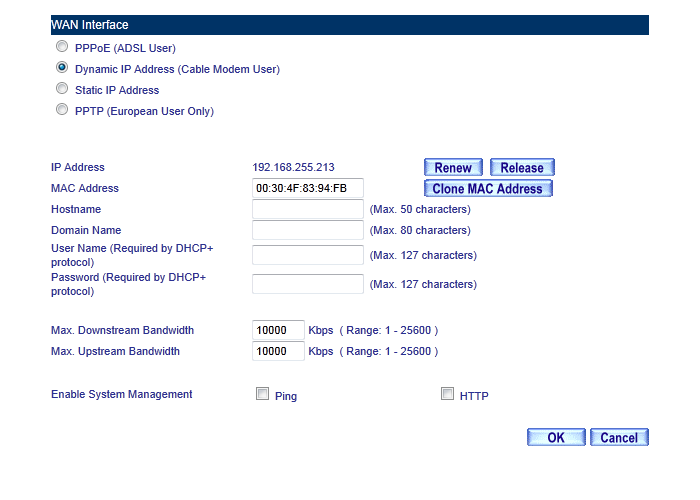
\includegraphics[width=\textwidth]{1.PNG}
    \end{center}
  \end{figure}


  \subsection{Zadanie 2}
  Menu konfiguracyjnym urządzenia nie różni się znacznie od menu domowych routerów.


  \subsection{Zadanie 3}
  \paragraph{}
  Ustawienie polisy umożliwiającej wyjście do Internetu.
  \begin{figure}[h!]
    \begin{center}
      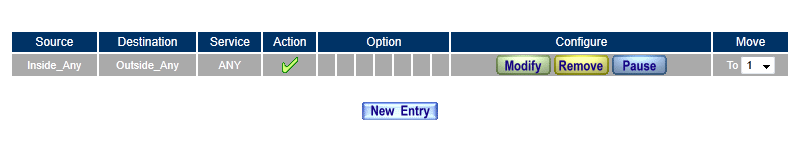
\includegraphics[width=\textwidth]{2.PNG}
    \end{center}
  \end{figure}

  Polisa umożliwiła dostep do internetu z obu komputerów.



  \subsection{Zadanie 4}
  \paragraph{}
  Zdefiniowane adresu 2 komputerów.
  \begin{figure}[h!]
    \begin{center}
      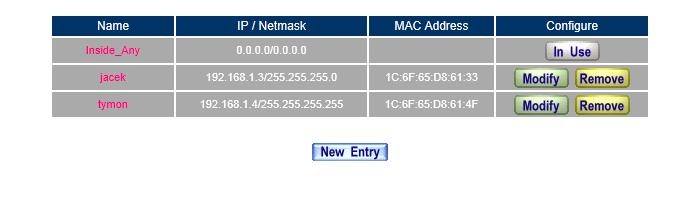
\includegraphics[width=\textwidth]{3.PNG}
    \end{center}
  \end{figure}


  \subsection{Zadanie 5}
  \paragraph{}
  Zdefiniowane reguły QoS.
  \begin{figure}[h!]
    \begin{center}
      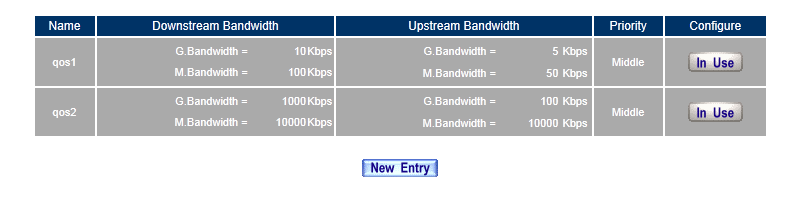
\includegraphics[width=\textwidth]{3_5.PNG}
    \end{center}
  \end{figure}


  \newpage
  \subsection{Zadanie 6}
  \paragraph{}
  Reguły ograniczające pasmo.

  \begin{figure}[h!]
    \begin{center}
      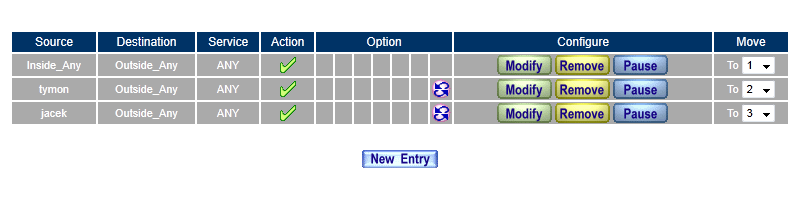
\includegraphics[width=\textwidth]{4.PNG}
    \end{center}
  \end{figure}

  \begin{figure}[h!]
    \begin{center}
      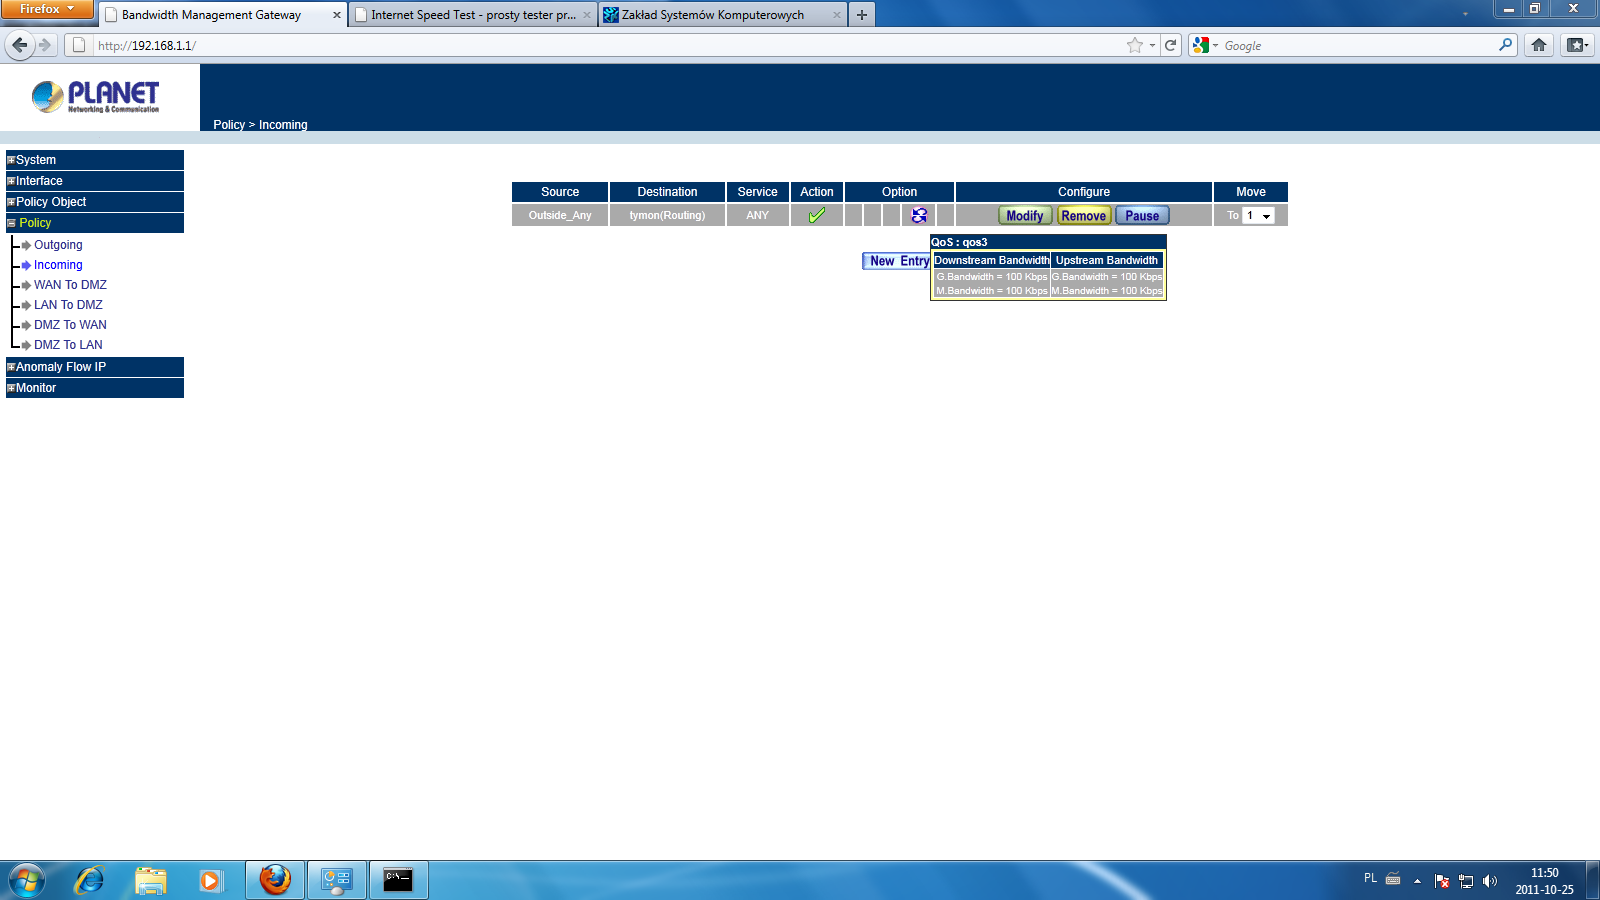
\includegraphics[width=\textwidth]{6.PNG}
    \end{center}
  \end{figure}

  \paragraph{}
  W celu sprawdzenia limitu pasma został wykorzystany serwis \textbf{http://speedtest.net}.
  \begin{figure}[h!]
    \begin{center}
      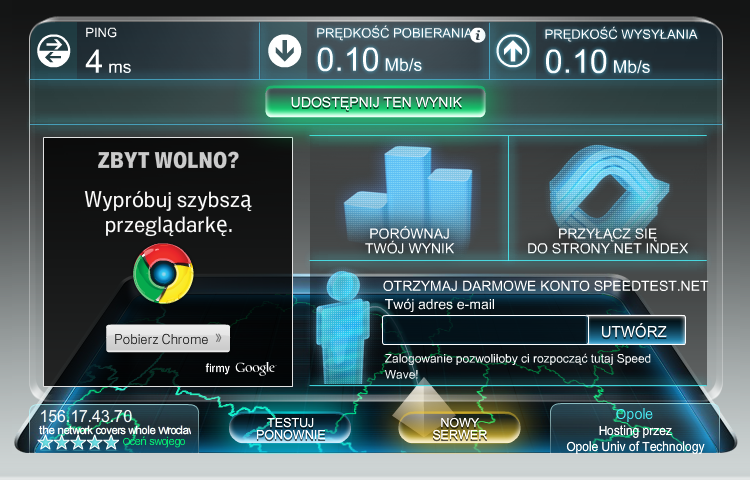
\includegraphics[width=\textwidth]{7.PNG}
    \end{center}
  \end{figure}

  Jak widać na wynikach testu pasmo zostało ograniczone do 100 Kb/s.

  \newpage

  \subsection{Zadanie 7}
  \paragraph{}
  Reguła blokująca pobieranie plików \textbf{.exe}.
  \begin{figure}[h!]
    \begin{center}
      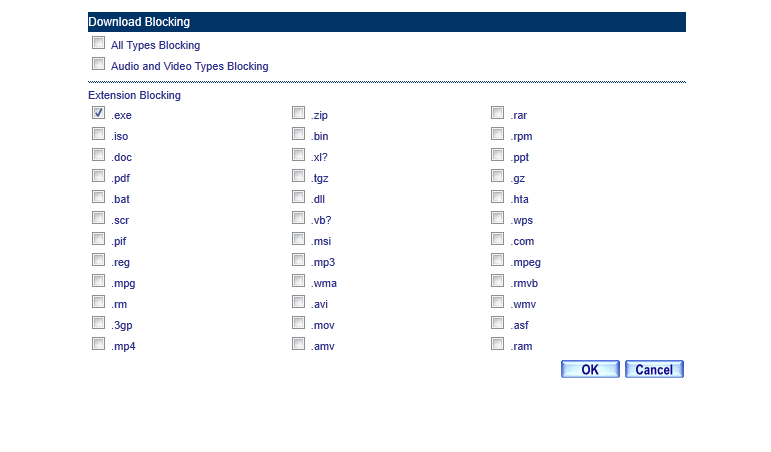
\includegraphics[width=\textwidth]{blocking_exe.PNG}
    \end{center}
  \end{figure}

  \paragraph{}
  Przetestowanie reguły blokującej pobieranie plików o rozszerzeniu \textbf{.exe}.
  \begin{figure}[h!]
    \begin{center}
      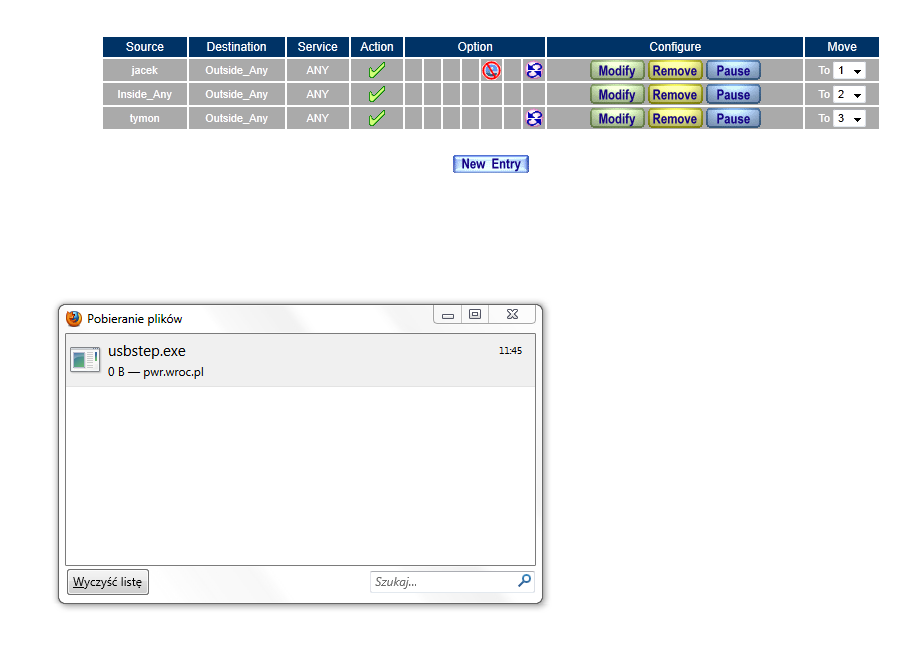
\includegraphics[width=\textwidth]{pobieranie_exe.PNG}
    \end{center}
  \end{figure}

  Jak widać manager pasma zablokował możliwość pobierania plików \textbf{.exe}.


  \subsection{Zadanie 8}
  \paragraph{}
  Reguła umożliwiająca połączenie jedynie ze stroną \textbf{kssk.pwr.wroc.pl}.
  \begin{figure}[h!]
    \begin{center}
      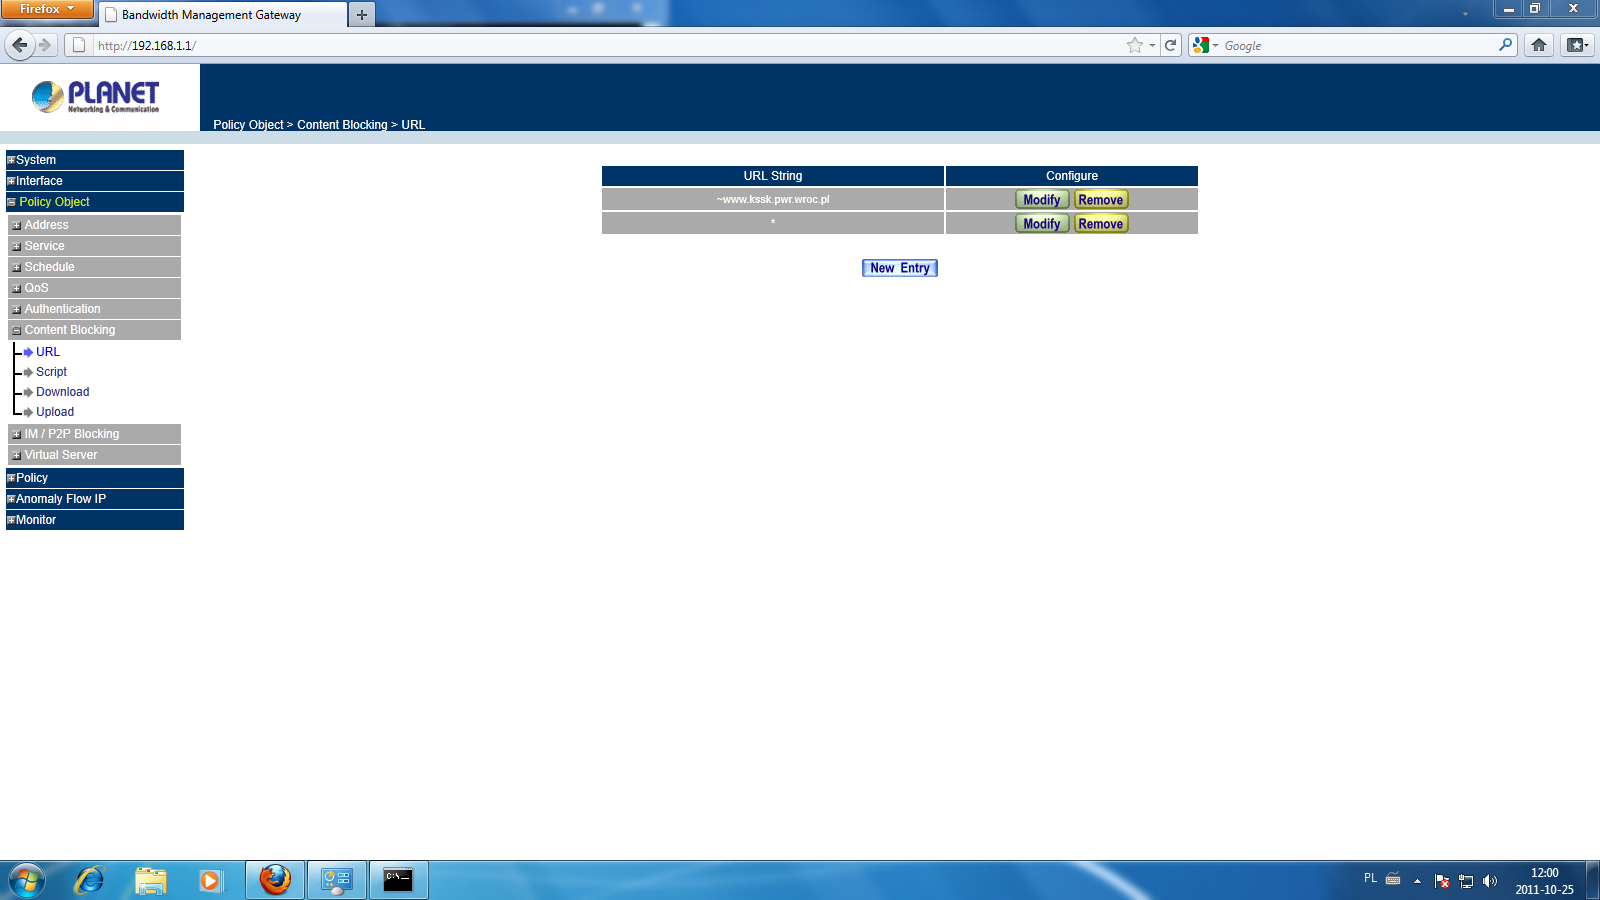
\includegraphics[width=\textwidth]{8.PNG}
    \end{center}
  \end{figure}

  Po zdefiniowaniu tej reguły inny strony internetowe stały się niedostępne dla użytkownika.


  \subsection{Zadanie 9}
  \paragraph{}
  Statystyki ruchu w sieci
  \begin{figure}[h!]
    \begin{center}
      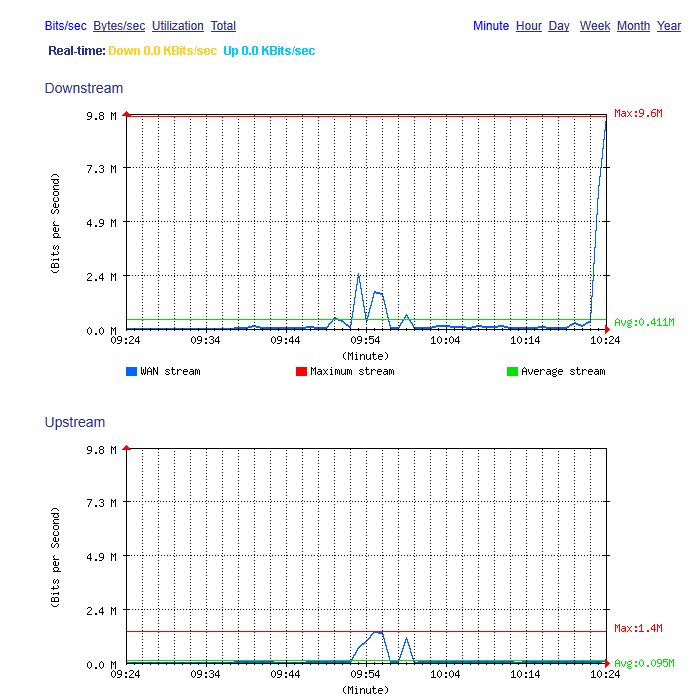
\includegraphics[width=\textwidth]{9.PNG}
    \end{center}
  \end{figure}


  \newpage
  \subsection{Zadanie 10}
  \paragraph{}
  Czasowe blokowanie domen.
  \begin{figure}[h!]
    \begin{center}
      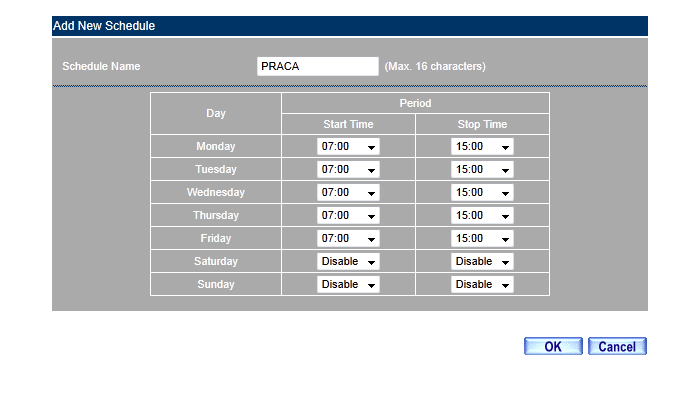
\includegraphics[width=\textwidth]{10.PNG}
    \end{center}
  \end{figure}
  \begin{figure}[h!]
    \begin{center}
      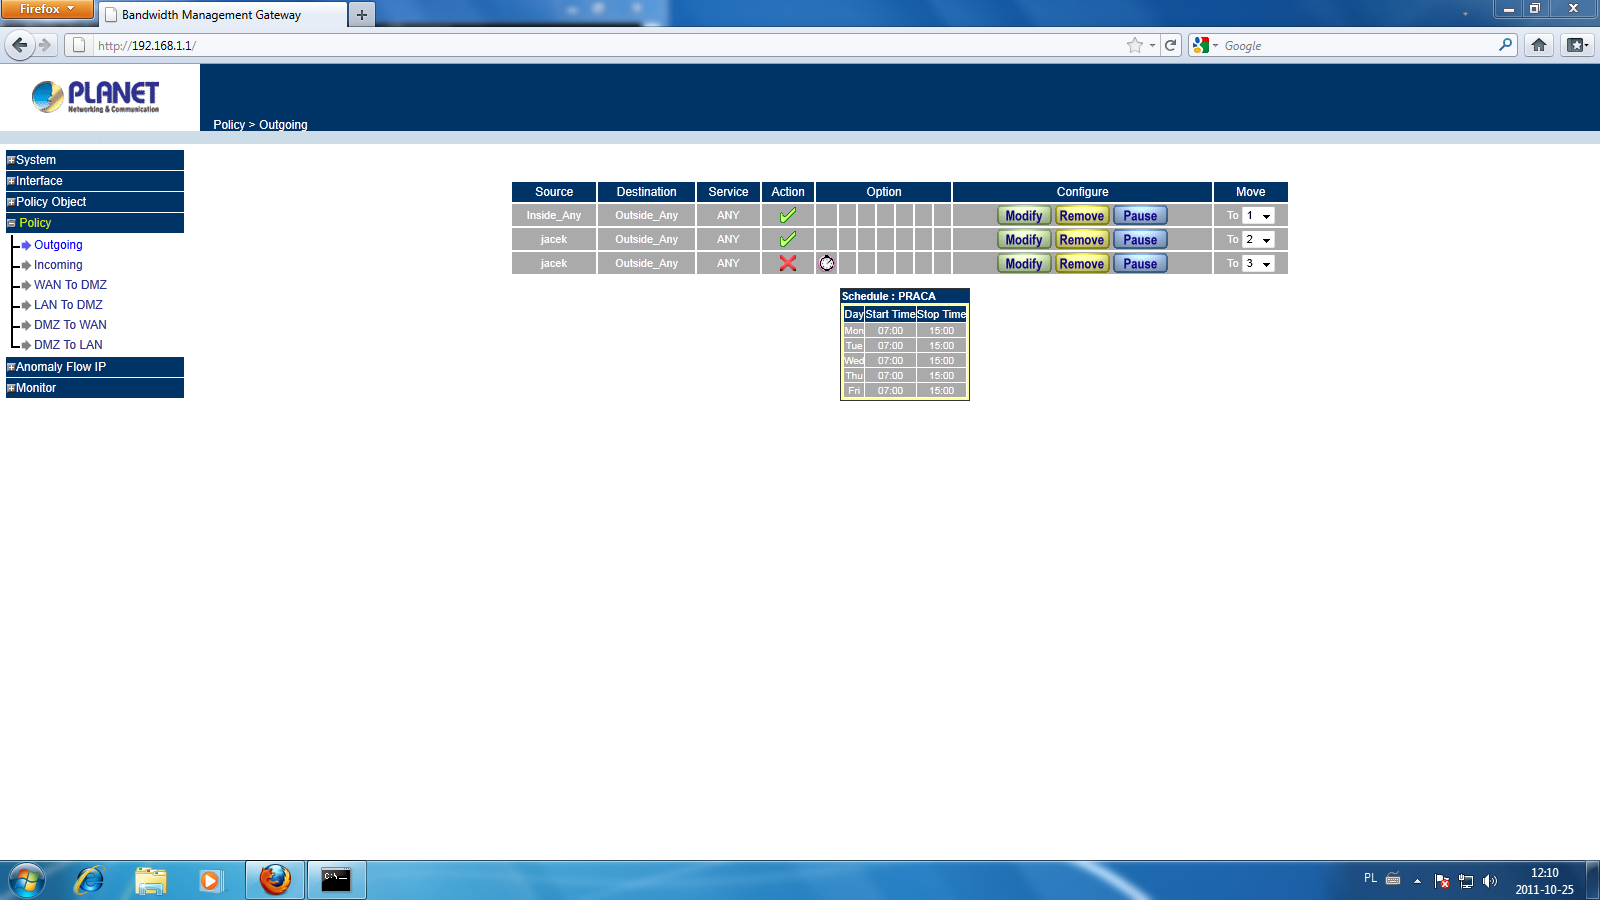
\includegraphics[width=\textwidth]{11.PNG}
    \end{center}
  \end{figure}

  \newpage
  \subsection{Zadanie 11}
  \paragraph{}
  Eksport ustawień routera do pliku.
  \begin{figure}[h!]
    \begin{center}
      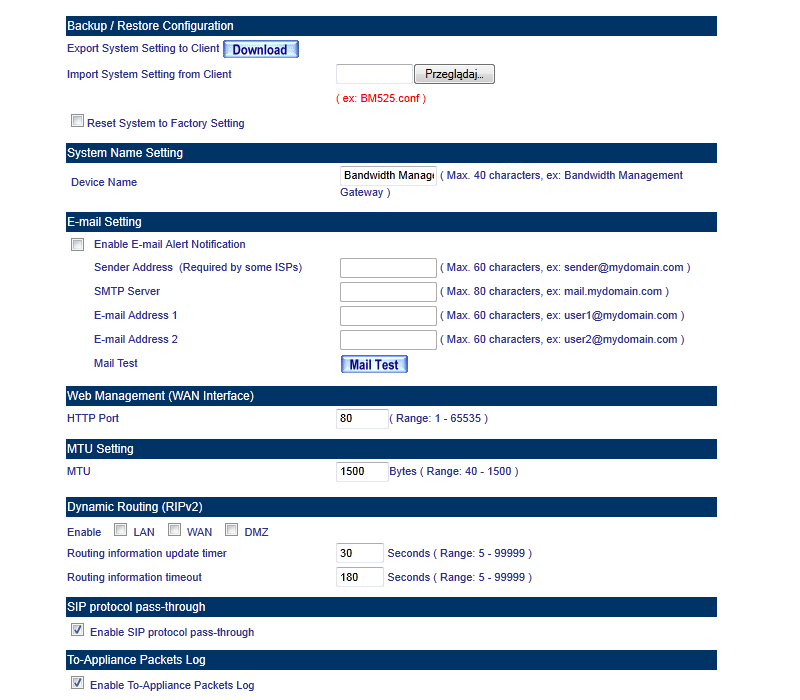
\includegraphics[width=\textwidth]{12.PNG}
    \end{center}
  \end{figure}

  \newpage
  \subsection{Zadanie 12}
  \paragraph{}
  Ustawienie automatycznej synchronizacji zegara z serwerem czasu rzeczywistego.
  \begin{figure}[h!]
    \begin{center}
      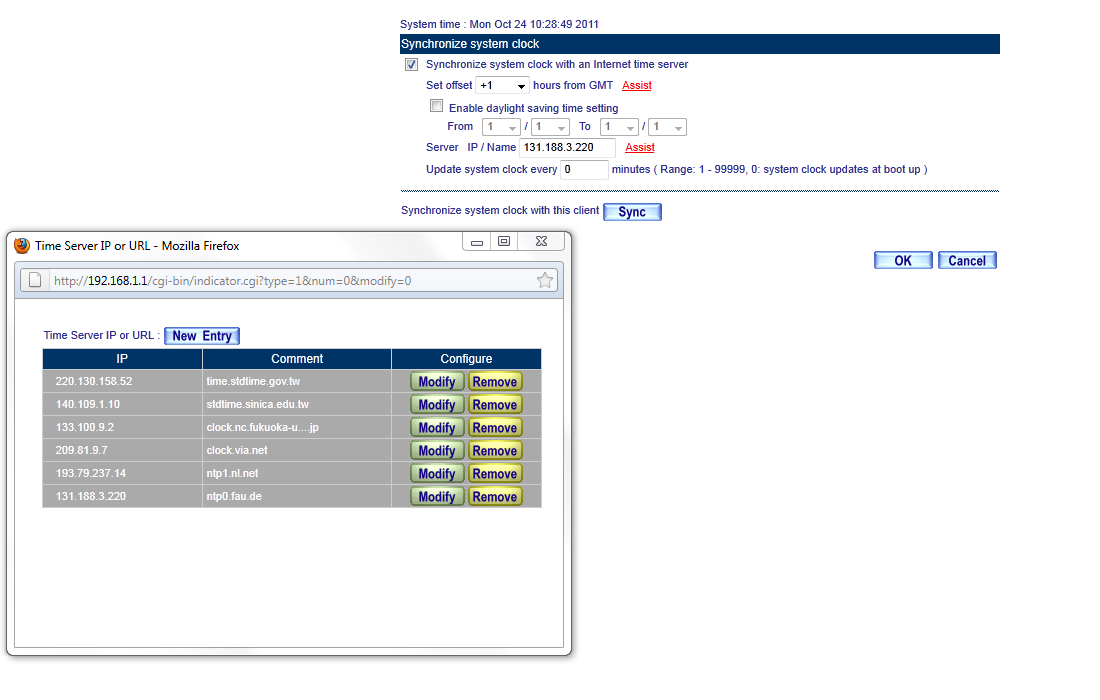
\includegraphics[width=\textwidth]{14.PNG}
    \end{center}
  \end{figure}


  \subsection{Zadanie 13}
  \paragraph{}
  Ustawienie priorytetu dla pakietów różnych usług.
  \begin{figure}[h!]
    \begin{center}
      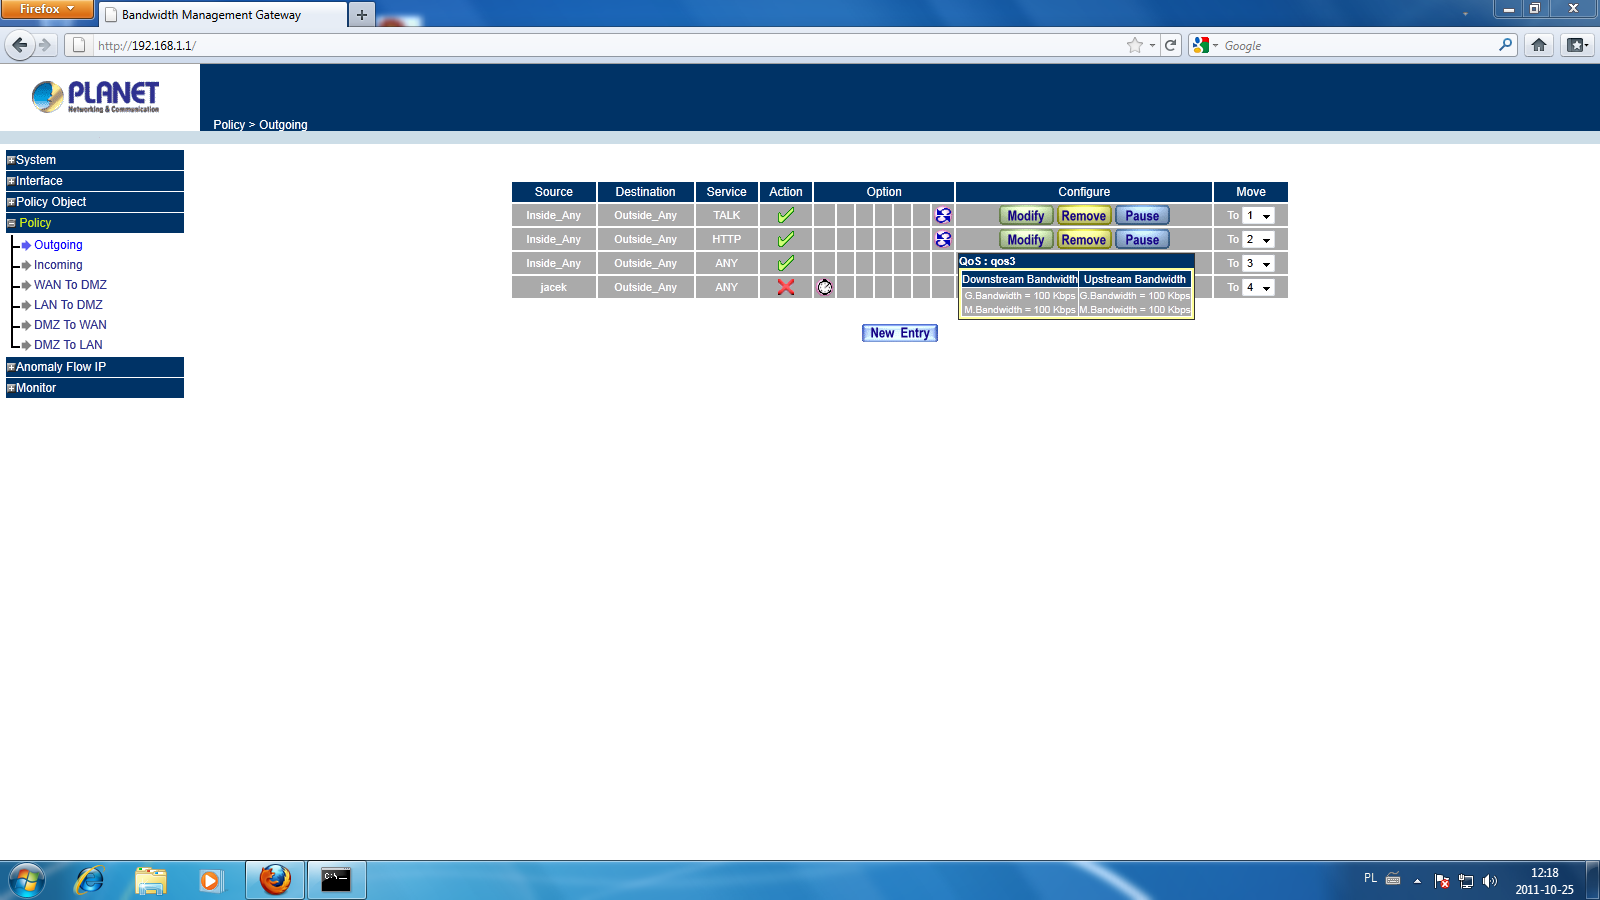
\includegraphics[width=\textwidth]{15.PNG}
    \end{center}
  \end{figure}

  \begin{figure}[h!]
    \begin{center}
      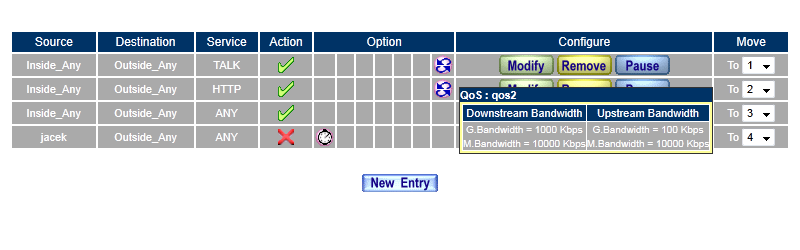
\includegraphics[width=\textwidth]{16.PNG}
    \end{center}
  \end{figure}



  \section{Wnioski}
  \paragraph{}
  Manager pasma BM525 posiada daje wiele możliwości zarządzania ruchem w sieci. Zapobiega on przeciążeniom oraz poprawia bezpieczeństwo. Pozwala on m.in. na przydzielenie poszczególnym urzytkownikom lub grupom urzytkowników limitu prędkości łącza, zablokowanie dostępu do określonych serwisów internetowych czy blokadę pobierania plików określonego typu. Ograniczenia mogą być też aktywowane tylko w określony przedziale czasu.

\end{document}